\subsection{Reduction example}\label{subsection:background:graphql:example-reduction}

This section contains a simple example of how query reduction is performed using apollo-augmented-hooks functionality inside the micro-frontend prototype. The client first navigates to a tabular view of all users. This page executes the GraphQL query shown in Listing \ref{code:applied-methods:query-all-users}. After fetching the query from the GraphQL \ac{API}, the fields in the query are cached in the Apollo Client's \texttt{InMemoryCache}.

\ifshowListings
  \begin{listing}[H]
  \begin{minted}{typescript}
query {
  allUsers {
    id
    username
    email
    password
    firstName
    secondName
    Title { id }
    Salutation { id }
  }
}
  \end{minted}
  \caption{A GraphQL query to fetch all users.}\label{code:applied-methods:query-all-users}
  \end{listing}
\fi

\noindent Afterwards, the client navigates to the detail view of a particular user. The left GraphQL query shown in Figure \ref{fig:applied-methods:comparison-user-reduced-user} is the original query that would normally be fetched from the GraphQL \ac{API} because the query name is different from the \texttt{allUsers} query. Using the functionality of removing fields from a query that are already cached, the query on the right in Figure \ref{fig:applied-methods:comparison-user-reduced-user} is sent to the GraphQL \ac{API}. The exact fields that were queried with the \texttt{allUsers} GraphQL query shown in Listing \ref{code:applied-methods:query-all-users} are removed from the \texttt{user} query. Therefore, 8 of the 16 fields are removed from the query, reducing the number of fields queried by 50\%. The following chapter explains in more detail the effects of reducing queries by using the \texttt{InMemoryCache}.

\ifshowImages
\begin{figure}[H]
  \centering
  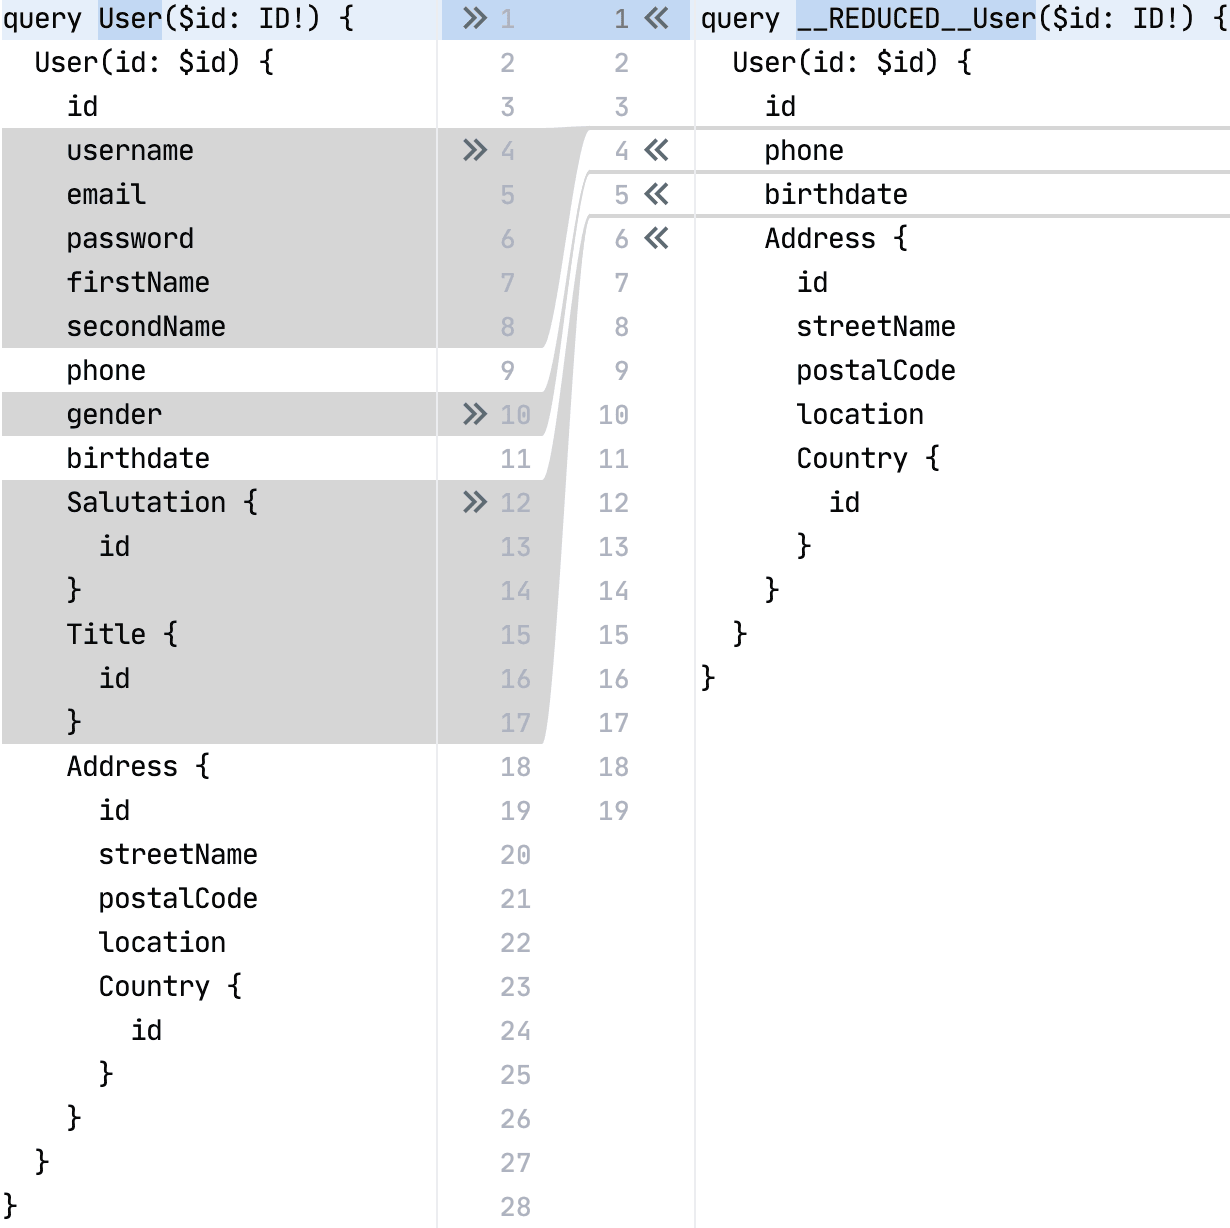
\includegraphics[width=0.65\linewidth]{images/reduction-graphql-examples/compare-user-reduced-user.png}
  \caption{A comparison of the original user- and reduced user-query.}\label{fig:applied-methods:comparison-user-reduced-user}
\end{figure}
\fi
